\documentclass[aspectratio=169, usenames, dvipsnames, 14pt]{beamer}
\usepackage[utf8]{inputenc}
\usepackage[utf8]{inputenc}
\usepackage{multirow}
\usepackage{gensymb}
\usepackage[absolute,overlay]{textpos}
\usepackage[export]{adjustbox}
\usepackage[absolute,overlay]{textpos}  % Absolute placement of text in frame

\usepackage{listings}           % For source code fonts
\usepackage{tikz}               % For absolute image placement and shapes
\usepackage{Formatting/python_formatting}   % User defined formatting file for source codes

\usepackage{Formatting/grid_overlay}        % Grid overlay for accurate placement of images
\usepackage{pstricks}
\usepackage{xcolor}

\usetikzlibrary{calc}           % For absolute image placement
\usetikzlibrary{decorations.pathreplacing}      % For curly braces

\usetikzlibrary{arrows, positioning, shapes.geometric}

\mode<presentation>
\usetheme{Rochester}

\title{\textbf{Getting derivatives in OpenMDAO}}
\author{John Jasa \and Justin Gray \\ \footnotesize johnjasa@umich.edu justin.s.gray@nasa.gov}
\institute{University of Michigan MDO Lab \and NASA Glenn Research Center}

\begin{document}

\begin{frame}

	\maketitle
	
	\tikz[remember picture, overlay] \node[anchor=center] at ($(current page.center)-(0, -3.7)$) {\includegraphics[scale=.24]{images/omdao.png}};
	
\end{frame}

\begin{frame}{Acknowledgement}
	
	\begin{itemize}
		\item \textbf{Ben Brelje}, PhD candidate at University of Michigan MDO lab for creating version 0 of this training
		\item \textbf{Justin Gray}, Engineer and team lead of OpenMDAO at NASA Glenn for refining this workshop
	\end{itemize}
	
\end{frame}

\begin{frame}{This session assumes some baseline knowledge}
	
	\begin{itemize}
		\item You've used OpenMDAO models before
		\item You understand when gradient-based optimization methods are advantageous
		\item You have a working understanding of how to differentiate equations by hand
	\end{itemize}
	
\end{frame}

\begin{frame}{Download these slides and tutorial scripts from GitHub}
	
	\url{https://github.com/openmdao/openmdao_training}
	\newline \newline Our materials for today are in the ``getting\_derivatives\_in\_openmdao'' folder
	\newline \newline This repo contains other tutorials to help you get acquainted with OpenMDAO
	
\end{frame}

\begin{frame}{Gradient-based optimization \underline{with analytic derivatives} is our only hope for large-scale problems}
	
	\begin{columns}
		\column[T]{0.5\textwidth}
			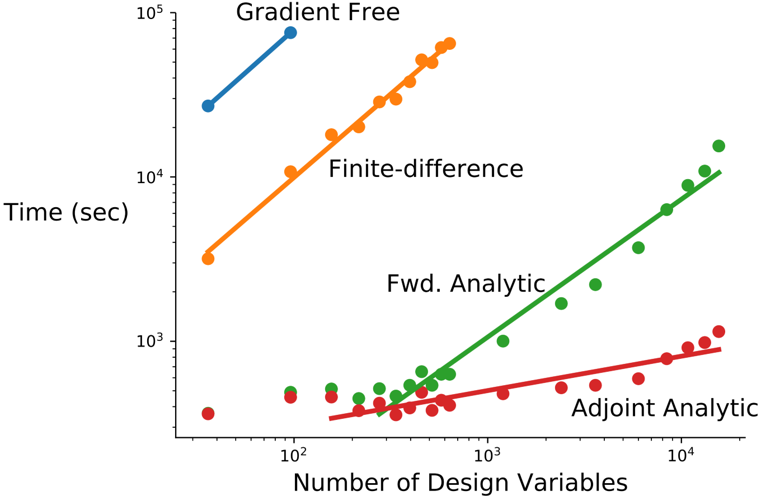
\includegraphics[scale=.35]{images/slide_5_derivatives.png}
		\column[T]{0.5\textwidth}
			\begin{itemize}
				\item 100x-10,000x speedup for aerodynamic shape optimization vs. gradient-free\textsuperscript{1}
				\item At least 5x-10x speedup vs. finite-difference \textsuperscript{2}
			\end{itemize}
			\footnotesize [1] Lyu et al. ICCFD8-2014-0203
			\footnotesize \newline [2] Gray et al. Aviation 2014-2042
	\end{columns}
	
\end{frame}
		
\begin{frame}{Goals for today}
	
	\begin{itemize}
		\item Understand how to obtain partial derivatives for your components
		\item Know the differences between explicit and implicit components and what that means for partials
		\item Briefly lear about some advanced techniques to obtain partial derivatives
	\end{itemize}

\end{frame}

\begingroup
\setbeamercolor{background canvas}{bg=GreenYellow}
\begin{frame}{Breif introduction to how OpenMDAO handles derivatives}

	\begin{itemize}
		\item Why do we need derivatives?
		\item How does OpenMDAO process these derivatives?
		\item How can we efficiently obtain these derivatives
	\end{itemize}

\end{frame}
\endgroup


\begin{frame}{Optimization}
    \begin{columns}
        \column[T]{0.5\textwidth}
            \begin{itemize}
                \item OpenMDAO is capable of evaluating DOEs and using gradient free methods, but…
                \item Gradient based optimization is A LOT faster! 
                \item So we need \textbf{total derivatives} across the whole model: 
            \end{itemize}
            
        \column[T]{0.5\textwidth}
            \begin{equation*}
                \hspace{-3cm} \vspace{-0.5cm} \frac{df(x)}{dx}
            \end{equation*}
            
            \begin{tikzpicture}[overlay, node distance = 0cm and 0.1cm]
                \tikzstyle{arrow} = [red, line width=1.5pt, ->, >=stealth]
                \tikzstyle{text_box} = [rectangle, minimum width=1cm, minimum height=1cm, text justified, fill= white!50]
                
                \node(image)    [text_box, xshift=3cm, yshift=-0.5cm] {\includegraphics[scale=0.2]{images/slide_70_image.PNG}};
                
                \node(eqn1)     [text_box, right of=image, node distance=3.4cm] {f(x)};
                
                \node(eqn2)     [text_box, below of=image, node distance=3.3cm] {$\displaystyle{\frac{df(x)}{dx}}$  \hspace{1cm} \textcolor{red}{??}};
                
                \node(circ1) [below of=eqn2, circle,red, thick, draw, minimum size=2cm, xshift=-1cm] (c) {};
                
                \draw [arrow]   (image) to (eqn1);
            \end{tikzpicture}
            
    \end{columns}
    
\end{frame}

\begin{frame}{Finite difference is easy}
    \begin{columns}
        \column[T]{0.5\textwidth}
            \small{
           \begin{equation*}
                {\frac{\partial F}{\partial x_{j}} = \frac{F(x+xe_{j}h) - F(x)}{h} + \theta (h)}
           \end{equation*}
        
            \vspace{1cm}
        
            f(x+h)      \hspace{.25cm}      + 1.2345678901234\textcolor{red}{31}\\
            f(x)        \hspace{.75cm}      + 1.234567890123456\\
            $\Delta f$    \hspace{1cm}        - 0.000000000000025
            }
        
        \column[T]{0.5\textwidth}
            \begin{tikzpicture}[overlay, node distance=0m and 0 cm]
                \tikzstyle{axes} = [black, line width = 1.5pt, ->, >=stealth]
                \tikzstyle{dotted} = [dashed]
                \tikzstyle{blueline} = [blue, thick]
                \tikzstyle{redline} = [red, thick]
                \tikzstyle{text_box} = [rectangle, minimum width=1cm, minimum height=1cm, text justified]
                
                % To move the image, change the 'yshift' value, and/or 'xshift'
                \node(origin) [circle, fill, inner sep=1.5pt, yshift=-4.5cm, xshift=1cm] {};
                \coordinate[above = 5cm of origin] (y);
                \coordinate[right = 5cm of origin] (x);
   
                \draw [axes]   (origin) to (y);
                \draw [axes]   (origin) to (x);
                
                % coordinates along x and y axes
                \coordinate [above = 2.5cm of origin]   (fx);
                \coordinate [above=0.75cm of origin]    (fxh);
                \coordinate [right=2cm of origin]       (x_cord);
                \coordinate [right=3.5cm of origin]     (xh);
                \coordinate [right=3.6cm of fxh]        (fxh_xh_int);
                
                % intersection point of curved line
                \node(int) [right=2cm of fx, circle, fill, inner sep=2pt] {};
                
                % dotted lines
                \draw[dotted] (fx) to (int);
                \draw[dotted] (int) to (x_cord);
                \draw[dotted] (fxh) to (fxh_xh_int);
                \draw[dotted] (xh) to (fxh_xh_int);
                
                % red line
                \draw[redline] (fxh_xh_int) to (int);
                
                % blue line
                \coordinate [below=2cm of int, xshift=0.7cm] (blue_bot);
                \coordinate [above=2cm of int, xshift=-0.7cm] (blue_top);
                \draw[blueline] (blue_bot) to (blue_top);
                
                % Curved plot
                \coordinate [above=2cm of fx, xshift=0.5cm] (top);
                \coordinate [right=1cm of xh, yshift=0.6cm] (bottom);
                \draw [very thick] (top) to [out=-20,in=110] (int) to [out=290,in=180] (bottom);
                
                 \node(y_fx) [text_box, left of=fx, node distance=0.5cm] {\footnotesize f(x)} {};
                 \node(y_fxh) [text_box, left of=fxh, node distance=0.75cm] {\footnotesize f(x+h)} {};
                 \node(xx) [text_box, below of=x_cord, node distance=0.3cm] {\footnotesize x} {};
                 \node(xxh) [text_box, below of=xh, node distance=0.3cm] {\footnotesize x+h} {};
                 
            \end{tikzpicture}
    \end{columns}
    
\end{frame}

 \begin{frame}{Finite difference is easy, but. . .} 
 
 \begin{columns}
     \column[T]{0.5 \textwidth}
         \begin{itemize}
             \item Treats your model as a black-box
             \item Expensive
             \item Accuracy can be bad, especially close to the optimal point
         \end{itemize}
 
         \vspace{-0.5cm}
 
         \begin{equation*}
             \frac{\partial \textbf{F}}{\partial x_{j}} =\frac{ \textbf{F}(\textbf{x}+e_{j}h)-\textbf{F(x)}}{h} +\Theta (h)
         \end{equation*}
 
     \column[T]{0.5 \textwidth}
     \includegraphics[scale=0.3]{images/slide73.png}
 
 \end{columns}
 
 \end{frame}
 
 \begin{frame}{It's not a good idea to finite difference across solvers}
\textbf{\small Seriously... Don’t do this unless you really have to.}

\begin{itemize}
    \item \small It’s expensive (make your solver tolerances really tight)
    \item \small It’s inaccurate
    \item \small It will probably make your optimization converge slowly!
\end{itemize}

\small Lots of papers on this topic: 

\tiny {
\begin{itemize}
\item \textbf{E. S. Hendricks and J. S. Gray, “Pycycle: a tool for efficient optimization of gas turbine engine cycles,”Aerospace, vol. 6, iss. 87, 2019.}

\item E. S. Hendricks, “A multi-level multi-design point approach for gas turbine cycle and turbine conceptual design,” PhD Thesis, 2017.

\item J. S. Gray, T. A. Hearn, K. T. Moore, J. Hwang, J. Martins, and A. Ning, “Automatic Evaluation of Multidisciplinary Derivatives Using a Graph-			Based Problem Formulation in OpenMDAO,” in15th AIAA/ISSMO Multidisciplinary Analysis and Optimization Conference, 2014.

\item J. S. Gray, K. T. Moore, T. A. Hearn, and B. A. Naylor, “Standard Platform for Benchmarking Multidisciplinary Design Analysis and Optimization Architectures,”AIAA Journal, vol. 51, iss. 10, p. 2380–2394, 2013.

\item C. Marriage and Martins, J. R. R. A. “Reconfigurable Semi-Analytic Sensitivity Methods and MDO Architectures Within the $\pi$MDO Framework”, in Proceedings of the 12th AIAA/ISSMO Multidisciplinary Analysis and Optimization Conference, Victoria, BC, 2008
\end{itemize}
}

\end{frame}

 \begin{frame}{Complex step is more accurate than FD, but}
     \begin{columns}
         \column[T]{0.5 \textwidth}
             \begin{itemize}
                 \item Treats your models as a gray-box (might require code modification)
                 \item Even more expensive
                 \item some functions are tricky ...
                     \begin{itemize}
                         \item min(), max(), abs() can cause issues
                     \end{itemize}
             \end{itemize}
 
             \vspace{-0.5cm}
 
             \begin{equation*}
                 \frac{\partial \textbf{F}}{\partial x_{j}} =\frac{Im(\textbf{F}(\textbf{x}+ihe_{j}))}{h} +\Theta (h^{2})
             \end{equation*}
 
         \column[T]{0.5 \textwidth}
             \includegraphics[scale=0.27]{images/slide75.png}
     \end{columns}
 
 \end{frame}    


 %---------------------------------------------------------------------%
 %---------------------------------------------------------------------%

 \begin{frame}{Analytic derivatives are both fast and accurate!}
 \begin{columns}
     \column[T]{0.5 \textwidth}
         \includegraphics[scale=0.25]{images/slide76.png}
 
     \column[T]{0.5 \textwidth}
         \vspace{2cm}
         \begin{equation*}
             \frac{df}{dx} = \frac{\partial f}{\partial y_{b}} \frac{\partial y_{b}}{\partial y_{a}} \frac{\partial y_{a}}{\partial x}
         \end{equation*}
 \end{columns}
 
 \end{frame}

 %---------------------------------------------------------------------%
 %---------------------------------------------------------------------%

 \begin{frame}{What about models with coupling?}
 \centering
 \includegraphics[scale=0.25]{images/slide77.png}
 
 \end{frame}

 %---------------------------------------------------------------------%
 %---------------------------------------------------------------------%

 \begin{frame}{How do you differentiate through this convergence loop? }
 \begin{columns}
     \column[T]{0.4 \textwidth}
         \includegraphics[scale=0.2]{images/slide78.png}
 
     \column[T]{0.6 \textwidth}
         \begin{itemize}
             \item We'll need a nonlinear solver to converge this coupling
             \vspace{0.5cm}
             \item The solver loop changes the way you compute analytic derivatives
         \end{itemize}
 \end{columns}
 
 \end{frame}

 %---------------------------------------------------------------------%
 %---------------------------------------------------------------------%
 \begin{frame}{Manually computing analytic derivatives for coupled models takes a lot of work}
 \begin{columns}
     \column[T]{0.35 \textwidth}
         \includegraphics[scale=0.2]{images/slide79.png}
 
     \column[T]{0.65 \textwidth}
 
        \begin{equation*}
             \frac{df}{dx} = \frac{\partial f}{\partial y_{b}} \frac{\partial y_{b}}{\partial y_{a}} \frac{\partial y_{a}}{\partial x} + \frac{\partial f}{\partial y_{b}} \frac{\partial y_{b}}{dx} + \frac{\partial y_{b}}{dx} + \frac{\partial f}{\partial y_{a}} \frac{dy_{a}}{dx}
         \end{equation*}
 \end{columns}
 
 \end{frame}

 %---------------------------------------------------------------------%
 %---------------------------------------------------------------------%

 \begin{frame}{How to compute these extra terms?}
 \begin{columns}
     \column[T]{0.35 \textwidth}
         \includegraphics[scale=0.2]{images/slide79.png}
 
     \column[T]{0.65 \textwidth}
 
        \begin{equation*}
             \frac{df}{dx} = \frac{\partial f}{\partial y_{b}} \frac{\partial y_{b}}{\partial y_{a}} \frac{\partial y_{a}}{\partial x} + \frac{\partial f}{\partial y_{b}} \frac{\partial y_{b}}{dx} + \frac{\partial y_{b}}{dx} + \frac{\partial f}{\partial y_{a}} \frac{dy_{a}}{dx}
         \end{equation*}
 
 
     \begin{tikzpicture}[overlay, node distance=0m and 0 cm]
         \tikzstyle{red_box} = [rectangle, draw, red, very thick, minimum width=0.7cm, minimum height=1.4cm, align=center]
         \tikzstyle{text_box} = [rectangle, minimum width=1cm, minimum height=1cm, text justified]
 
         \node(text) [text_box, yshift=-2.5cm, xshift=4.5cm] {\textcolor{red}{These terms will be computed using adjoints!}};
 
         %  to shift red boxes, move only box 1, the lines will follow
         \node(box1) [red_box, above of=text,  node distance=3.7cm, xshift=2.2cm] {};
         \node(box2) [red_box, right of=box1,  node distance=2cm] {};
 
         \draw[red, thick] (text) -- (box1);
         \draw[red, thick] (text) -- (box2);
 \end{tikzpicture}
 \end{columns}
 
 \end{frame}
 
 \begin{frame}{When models get really big, have fun!}
\begin{columns}
    \column[T]{0.6 \textwidth}
        \includegraphics[scale=0.5]{images/slide_81.png}
    
    \column[T]{0.4 \textwidth}
        \begin{center}
            
        
        \begin{equation*}
            \LARGE\frac{df}{dx} = ???
        \end{equation*}
        \end{center}
        Lets be honest, this is just not going to happen
    
\end{columns}
    
\end{frame}

%---------------------------------------------------------------------%
%---------------------------------------------------------------------%

\begin{frame}{OpenMDAO can compute these total derivatives for you, automatically!}
\begin{columns}
    \column[T]{0.5 \textwidth}
        \includegraphics[scale=0.5]{images/slide_81.png}
    
    \column[T]{0.5 \textwidth}
        \begin{center}

        \begin{equation*}
            \LARGE\frac{df}{dx} = [ask OpenMDAO]
        \end{equation*}
       
    \textbf{For a deep dive on the math}
            \begin{itemize}
                \item Martins and Hwang 2013
                \item Hwang and Martins 2018 
            \end{itemize}
        \end{center}
\end{columns}
    
\end{frame}

%---------------------------------------------------------------------%
%---------------------------------------------------------------------%


\begin{frame}{OpenMDAO splits total derivative computation into two steps}
\begin{columns}
    \column[T]{0.4 \textwidth}
        \includegraphics[scale=0.2]{images/slide76.png}
        
    \column[T]{0.6 \textwidth}
         1) Computing the partial derivatives for each component \newline \newline
         2) Solving a linear system for total derivatives
\end{columns}
    
\end{frame}

%---------------------------------------------------------------------%
%---------------------------------------------------------------------%

\begin{frame}{OpenMDAO splits total derivative computation into two steps}
	\begin{columns}
		\column[T]{.4 \textwidth}
			\includegraphics[scale=0.2]{images/slide76.png}
	
		\column[T]{.6 \textwidth}
			\textbf{1) Computing the partial derivatives for each component}
					\begin{itemize}
						\item Numerical approach: FD/CS
						\item Analytic approach: hand derivation or algorithmic differentiation
						\item Mix and match numerical and analytic
					\end{itemize}
			\text{You are responsible for this step,} 
			\text{but OpenMDAO can help you a bit}
	\end{columns}

	\begin{tikzpicture}[overlay]
		\draw[red, very thick, ->] (5.5, 5.5) to (0.2, 4.7);
		\draw[red, very thick, ->] (5.5, 5.5) to (1.1, 3.3);
		\draw[red, very thick, ->] (5.5, 5.5) to (2.0, 2.1);
	\end{tikzpicture}

\end{frame}

\begin{frame}{OpenMDAO splits total derivative computation into two steps}
	\begin{columns}
		\column[T]{.4 \textwidth}
			\includegraphics[scale=0.2]{images/slide76.png}
	
		\column[T]{.6 \textwidth}
			1) Computing the partial derivatives for each component \newline \newline
			\textbf{2) Solving a linear system for total derivatives}
			\newline \newline
			OpenMDAO does this automatically using a library of different linear solvers for different problems
	\end{columns}

	\begin{tikzpicture}[overlay]
		\draw[blue, ultra thick] (0.1, 4.8) to ( 0.1, 4.1);
		\draw[blue, ultra thick] (0.1, 4.1) to ( 1, 4.1);
		\draw[blue, ultra thick] (1, 4.1) to ( 1, 2.8);
		\draw[blue, ultra thick] (1, 2.8) to ( 2, 2.8);
		\draw[blue, ultra thick] (2, 2.8) to ( 2, 1.55);
		\draw[blue, ultra thick] (2, 1.55) to ( 2.8, 1.55);
	\end{tikzpicture}
\end{frame}

\begin{frame}{By using OpenMDAO's analytic derivative functionality you can}
	\begin{itemize}
		\item Efficiently solve optimization problems with thousands of design variables or thousands of constraints
		\item Get total derivatives across a complicated model by providing only partial derivatives of each componFent
		\item Mix and match different techniques for computing partial derivatives
	\end{itemize}
\end{frame}

\begin{frame}{OpenMDAO docs have a great amount of details and examples}

	\begin{columns}
		\column[T]{.5\textwidth}
			Search bar is a lifesaver
			\newline \newline \newline \newline \url{http://openmdao.org/twodocs/versions/latest/features/core_features/working_with_derivatives/index.html}
		\column[T]{.5\textwidth}
			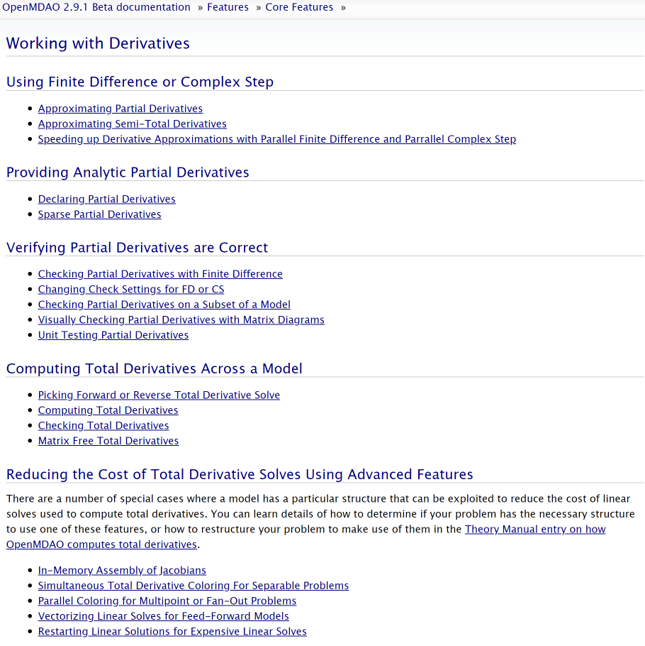
\includegraphics[scale=.37]{images/slide_24_derivatives.png}
	\end{columns}

\end{frame}

\begin{frame}{OpenMDAO docs have a great amount of details and examples}

	\begin{figure}
		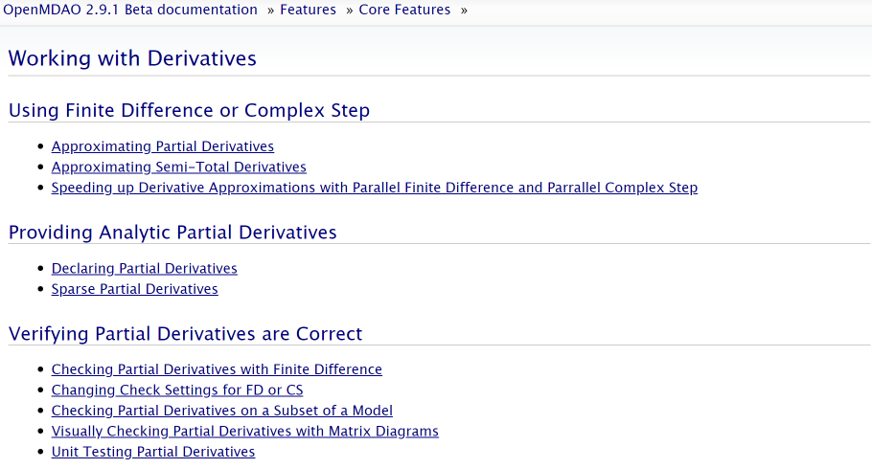
\includegraphics[scale=.4]{images/slide_25_derivatives.png}
	\end{figure}
	\url{http://openmdao.org/twodocs/versions/latest/features/core_features/working_with_derivatives/index.html}
	
\end{frame}

\begingroup
\setbeamercolor{background canvas}{bg=GreenYellow}
\begin{frame}{Computing partial derivatives of an ExplicitComponent}

	\begin{itemize}
		\item Hand-derived
		\item Sparse hand-derived
		\item Approximated (finite-difference or complex-step)
		\item Under the ``explicit\_examples'' folder in the repo
	\end{itemize}

\end{frame}
\endgroup

\begin{frame}{ExplicitComponent class}
    \begin{columns}[T]
  
        \column{0.5 \textwidth}
            \begin{itemize}
                \item Used for doing explicit calculations
                \vspace{.5cm}
                \item Inputs $\rightarrow$ Outputs
                \vspace{.5cm}
                \item Can be as simple as a one-line calculation, or as complex as an adjoint CFD solver
            \end{itemize}

    \column{0.5 \textwidth}
        \begin{tikzpicture}[overlay]
            % \draw (2.9, -2) node [inner sep=0] {\uncover<1->{\includegraphics[scale=0.2]{images/arch1.png};}};
            \draw (2.9, -2) node [inner sep=0] {\includegraphics[scale=0.2]{images/arch1.png}};
            \draw [blue, ultra thick] (4.8,-2.7) circle (0.65cm);
            \draw[blue, very thick] (-2,1.3) -- (4.2, -2.5);
        \end{tikzpicture}
  \end{columns}
 
\end{frame}

\begin{frame}{A simple ExplicitComponent example: Calculating lift from C\textsubscript{L}}

	\begin{equation}
		\large L = \frac{1}{2} C_L \rho V^2 S_{ref}
	\end{equation}
	
\end{frame}

\begin{frame}{You can analytically compute the partials by hand}

	\begin{columns}
		\column[T]{.5\textwidth}
			\begin{equation}
				\large L = \frac{1}{2} C_L \rho V^2 S_{ref}
			\end{equation}
		\column[T]{.5\textwidth}
			\begin{equation}
				\small \frac{\partial L}{\partial V} = C_L \rho V S_{ref} 
			\end{equation}
			\begin{equation}
				\small \frac{\partial L}{\partial C_L} = \frac{1}{2} \rho V^2 S_{ref}
			\end{equation}
			\begin{equation}
				\small \frac{L}{\rho} = \frac{1}{2} C_L V^2 S_{ref}
			\end{equation}
			\begin{equation}
				\small \frac{\partial L}{\partial S_{ref}} = \frac{1}{2} C_L \rho V^2
			\end{equation}
	\end{columns}

\end{frame}

\begin{frame}{OpenMDAO can approximate partial derivatives for you}

	\begin{itemize}
		\item Can use the finite-difference or compelx-step methods to approximate the partial derivatives
		\item This is generally more computationally expensive than anlytic derivatives
		\item It requires very little additional programmer time
	\end{itemize}

\end{frame}

\begin{frame}

	\tikz[remember picture, overlay] \node[anchor=center] at ($(current page.center)-(0, 0)$) {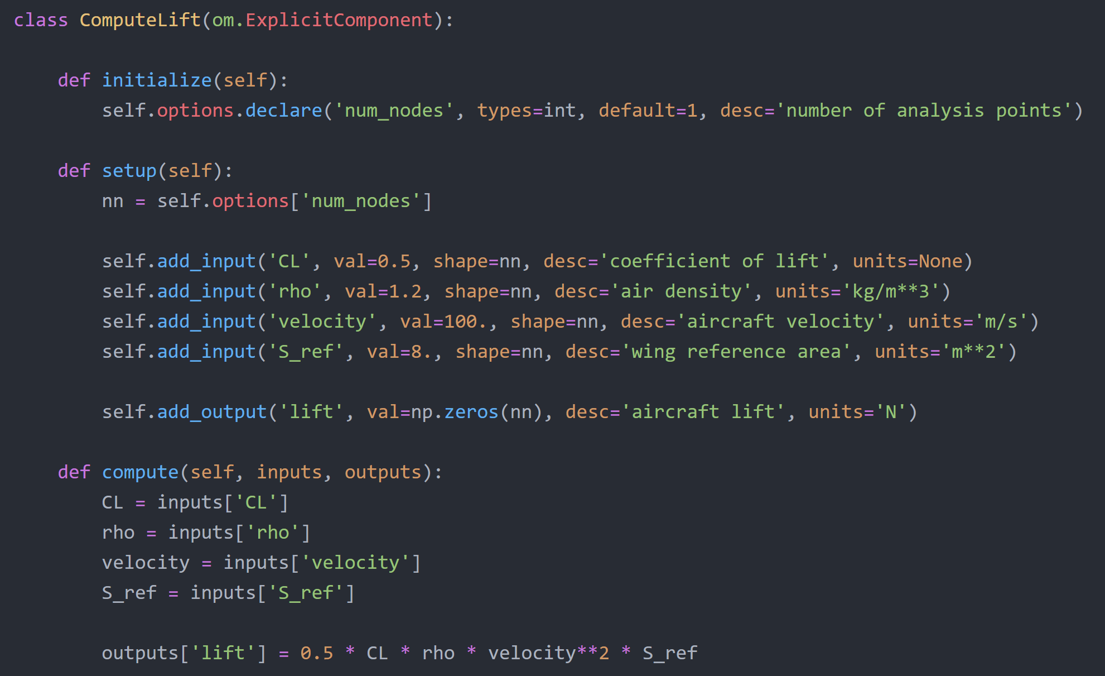
\includegraphics[scale=.5]{images/slide_31_derivatives.png}};
	
	\begin{textblock*}{4cm}(9cm, 6.6cm)
		\textcolor{white}{$ L = \dfrac{1}{2} C_L \rho V^2 S_{ref} $}
	\end{textblock*}
	
\end{frame}

\begin{frame}

	\tikz[remember picture, overlay] \node[anchor=center] at ($(current page.center)-(0, -.6)$) {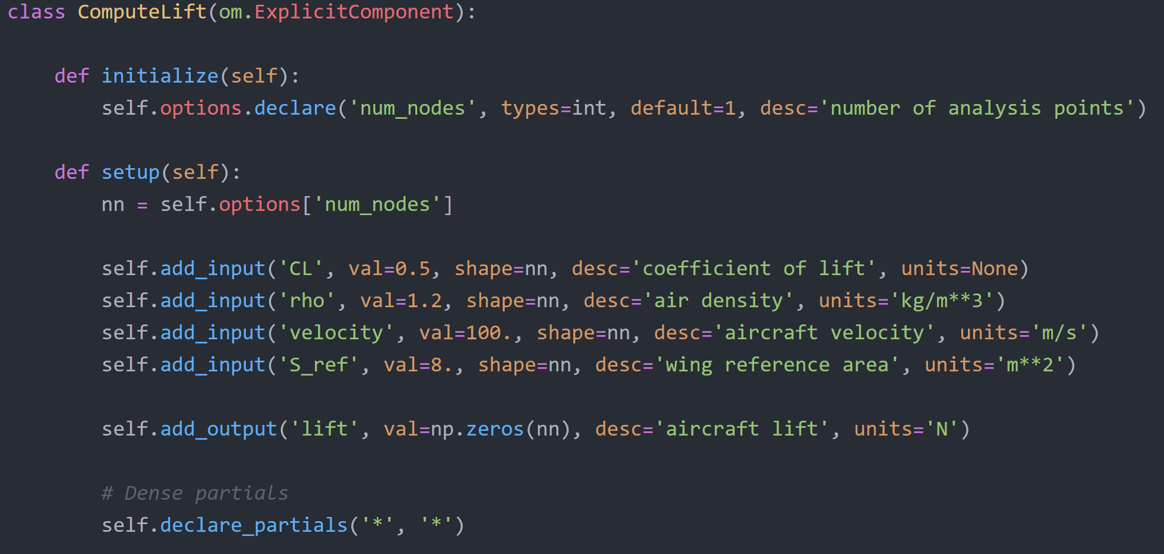
\includegraphics[scale=.525]{images/slide_32_derivatives.png}};
	
	\begin{textblock*}{15cm}(2cm, 8cm)
		We tell OpenMDAO that all outputs depend on all inputs
	\end{textblock*}
	
	\begin{tikzpicture}[overlay]
		\draw[white, thick, ->] (8.3, -2.15) to (5.7, -2.15);
	\end{tikzpicture}
	
\end{frame}

\begin{frame}{The Jacobian is a matrix with one row for each output, and one column for each input}

	$$
	[J] = 
	\begin{bmatrix}
		\frac{\partial L}{\partial V} & \frac{\partial L}{\partial C_L} & \frac{\partial L}{\partial \rho} & \frac{\partial L}{\partial S_{ref}}
	\end{bmatrix}
	$$

\end{frame}

\begin{frame}{But each entry is that matrix is really a sub-matrix!}

	\begin{itemize}
		\item Each input is really a vector
		\item Each output is really a vector
		\item Each entry of the vector is totally separate from all others
		\item So each partial is really a square matrix, with entries only on the diagonal
	\end{itemize}
	$$
	[J] = 
	\begin{bmatrix}
		\frac{\partial L}{\partial V} & \frac{\partial L}{\partial C_L} & \frac{\partial L}{\partial \rho} & \frac{\partial L}{\partial S_{ref}}
	\end{bmatrix}
	$$
	
\end{frame}

\begin{frame}{But each entry in that matrix is really a sub-matrix!}

	$$
	\large [J] = 
	\begin{bmatrix}
		\frac{\partial L}{\partial V} & \frac{\partial L}{\partial C_L} & \frac{\partial L}{\partial \rho} & \frac{\partial L}{\partial S_{ref}}
	\end{bmatrix}
	$$	
	
	\tikz[remember picture, overlay] \node[anchor=center] at ($(current page.center)-(3.25, 3.0)$) {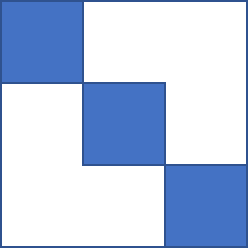
\includegraphics[scale=.24]{images/slide_35a_derivatives.png}};
		
	\tikz[remember picture, overlay] \node[anchor=center] at ($(current page.center)-(.75, 3.0)$) {
\includegraphics[scale=.24]{images/slide_35b_derivatives.png}};
	
	\tikz[remember picture, overlay] \node[anchor=center] at ($(current page.center)-(-1.75, 3.0)$) {
\includegraphics[scale=.24]{images/slide_35c_derivatives.png}};
				
	\tikz[remember picture, overlay] \node[anchor=center] at ($(current page.center)-(-3.75, 3.0)$) {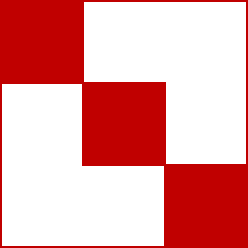
\includegraphics[scale=.24]{images/slide_35d_derivatives.png}};
	
	\begin{tikzpicture}[overlay]
		\draw[red, thick, ->] (3.75, 1) to (6, 3);
		\draw[red, thick, ->] (6.25, 1) to (7, 3);
		\draw[red, thick, ->] (8.75, 1) to (8, 3);
		\draw[red, thick, ->] (10.75, 1) to (9, 3);
	\end{tikzpicture}
	
\end{frame}

\begin{frame}

	\tikz[remember picture, overlay] \node[anchor=center] at ($(current page.center)-(0, 0)$) {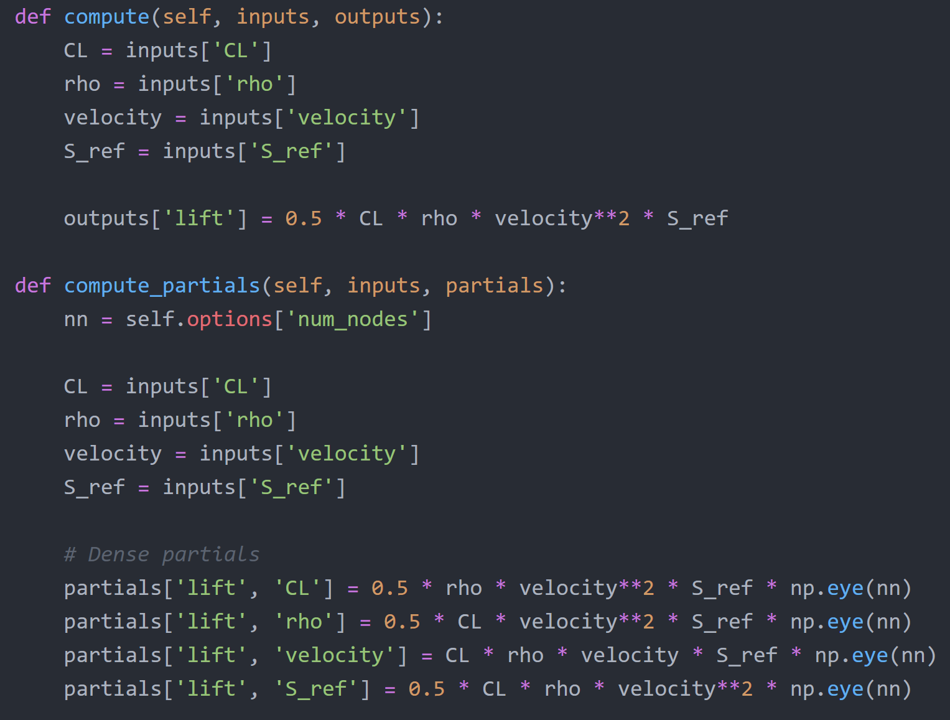
\includegraphics[scale=.475]{images/slide_36_derivatives.png}};
	
	\begin{textblock*}{8cm}(7.25cm, 4.5cm)
		\textcolor{white}{\footnotesize Give OpenMDAO the expressions for partial derivatives we computed before \newline \newline Account for the 			shape of the 	Jacobian}
	\end{textblock*}
	
\end{frame}

\begin{frame}{check\_partials output}
	
	\tikz[remember picture, overlay] \node[anchor=center] at ($(current page.center)-(0, 1.12)$) {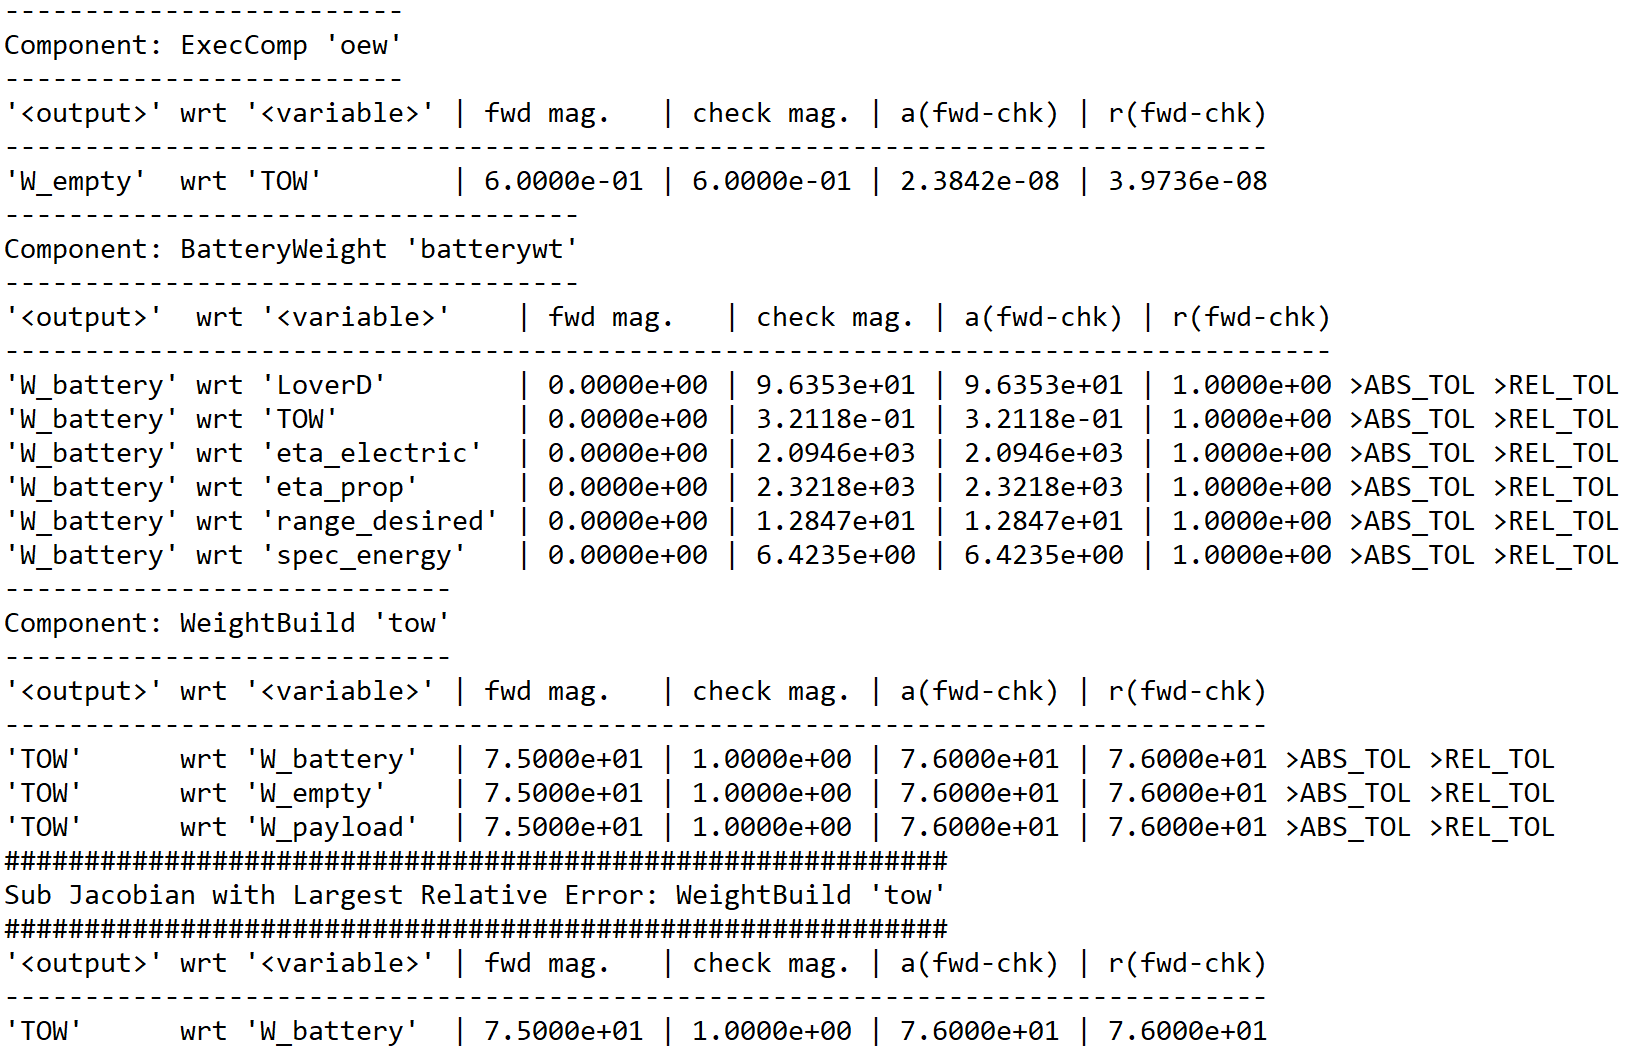
\includegraphics[scale=.485]{images/slide_37_derivatives.png}};
	
\end{frame}                                                                                                                                               

\end{document}